\documentclass{beamer}
\usetheme{tokitex}

\usepackage{tikz}
\usepackage{graphics}
\usepackage{multirow}
\usepackage{tabto}

\usepackage[english,bahasa]{babel}
\newtranslation[to=bahasa]{Section}{Bagian}
\newtranslation[to=bahasa]{Subsection}{Subbagian}

\usepackage{listings, lstautogobble}
\usepackage{color}

\definecolor{dkgreen}{rgb}{0,0.6,0}
\definecolor{gray}{rgb}{0.5,0.5,0.5}
\definecolor{mauve}{rgb}{0.58,0,0.82}

\lstset{frame=tb,
  language=c++,
  aboveskip=1mm,
  belowskip=1mm,
  showstringspaces=false,
  columns=fullflexible,
  keepspaces=true,
  basicstyle={\small\ttfamily},
  numbers=none,
  numberstyle=\tiny\color{gray},
  keywordstyle=\color{blue},
  commentstyle=\color{dkgreen},
  stringstyle=\color{mauve},
  breaklines=true,
  breakatwhitespace=true,
  autogobble=true
}

\usepackage{caption}
\captionsetup[figure]{labelformat=empty}

\newcommand{\progTerm}[1]{\texttt{#1}}
\newcommand{\foreignTerm}[1]{\textit{#1}}
\newcommand{\newTerm}[1]{\alert{\textbf{#1}}}
\newcommand{\emp}[1]{\alert{#1}}
\newcommand{\statement}[1]{"#1"}


\title{\textit{Masukan/Keluaran}}
\author{Tim Olimpiade Komputer Indonesia}
\date{}

\begin{document}

\begin{frame}
\titlepage
\end{frame}

\section{Masukan}
\frame{\sectionpage}

\begin{frame}[fragile]
\frametitle{Kilas Balik: kuadrat.cpp}
\begin{itemize}
  \item Sekarang coba lihat kembali program kuadrat.cpp:
\begin{lstlisting}
#include <cstdio>

int a, b, c, x, hasil;

int main() {
  a = 1;
  b = 3;
  c = -2;
  x = 2;

  hasil = a*x*x + b*x + c;
  printf("ax^2 + bx + c = %d\n", hasil);
}\end{lstlisting}
  \item Jika kita ingin mengganti nilai \texttt{x}, kode harus diganti, dikompilasi ulang, baru dijalankan kembali.
  \item Untuk menghasilkan keluaran yang bervariasi, perlu ada \newline masukan dari luar program.
\end{itemize}
\end{frame}

\begin{frame}
\frametitle{Membaca Masukan}
\begin{itemize}
  \item Diperlukan mekanisme untuk melakukan pembacaan masukan dari luar program.
  \item Masukan bagi suatu program bisa berasal dari berbagai sumber, misalnya \textit{standard input} atau \textit{file}.
  \item Kita akan mempelajari fungsi yang umum untuk membaca masukan, yaitu \emp{scanf}.
\end{itemize}
\end{frame}

\begin{frame}[fragile]
\frametitle{Membaca Masukan: scanf}
\begin{itemize}
  \item Modifikasi bagian \texttt{x = 2} menjadi \texttt{scanf("\%d", \&x)}:
\begin{lstlisting}
#include <cstdio>

int a, b, c, x, hasil;

int main() {
  a = 1;
  b = 3;
  c = -2;
  scanf("%d", &x);

  hasil = a*x*x + b*x + c;
  printf("ax^2 + bx + c = %d\n", hasil);
}
\end{lstlisting}
  \item Kompilasi, dan jalankan program. Kemudian ketikkan angka 2, dan tekan enter.
  \item Selamat! Kalian berhasil membaca masukan!
\end{itemize}
\end{frame}

\begin{frame}[fragile]
\frametitle{Fungsi scanf}
  \begin{itemize}
    \item Fungsi \textbf{scanf} berguna untuk membaca masukan, dan nilainya dapat di-\textit{assign} ke dalam variabel.
    \item Fungsi ini disediakan oleh STL cstdio.
    \item Cara kerja scanf: pada berkas masukan, cari \textit{token} yang dapat dibaca berikutnya, lalu baca ambil nilainya.
    \item Yang dimaksud \textit{token} adalah serangkaian karakter non-spasi, misalnya huruf atau angka.
    \item Pada contoh sebelumnya, \textit{token} yang dimaksud adalah bilangan yang akan menjadi nilai variabel \texttt{x}.
  \end{itemize}
\end{frame}


\begin{frame}[fragile]
\frametitle{Fungsi scanf (lanj.)}
  \begin{itemize}
    \item Sama dengan \texttt{printf}, diperlukan simbol sesuai tipe data yang bersangkutan.
    \item Perbedaan paling mendasar adalah diperlukannya karakter '\&' pada variabel yang hendak diisi.
  \end{itemize}
\end{frame}

\begin{frame}[fragile]
\frametitle{Membaca Beberapa Variabel}
  \begin{itemize}
    \item Hal ini juga berlaku apabila Anda hendak membaca beberapa variabel pada satu baris masukan.
\begin{lstlisting}
#include <cstdio>

int a, b, c, x, hasil;

int main() {
  scanf("%d %d %d %d", &a, &b, &c, &x);

  hasil = a*x*x + b*x + c;
  printf("ax^2 + bx + c = %d\n", hasil);
}
\end{lstlisting}    
    \item Jalankan program lalu masukkan "1 3 -2 2", lalu tekan enter.
  \end{itemize}
\end{frame}

\begin{frame}[fragile]
\frametitle{Membaca Beberapa Variabel (lanj.)}
  \begin{itemize}
    \item Meskipun kita memberikan pola "\texttt{\%d \%d \%d \%d}", tidak masalah apabila masukan yang hendak Anda baca ada di baris yang berbeda.
    \item Misalnya Anda dapat ketikkan "1 3", enter, "-2 2", lalu enter.
    \item Masukan tetap akan dibaca sesuai urutan yang diberikan.
    \item Alasannya adalah scanf membaca bilangan dengan cara mencari \foreignTerm{token} yang ada selanjutnya, tanpa peduli baris baru atau spasi.
  \end{itemize}
\end{frame}

\begin{frame}[fragile]
\frametitle{Membaca Karakter}
  \begin{itemize}
    \item Terkecuali pada tipe data karakter, scanf \emp{tidak} membaca \foreignTerm{token} selanjutnya.
    \item Scanf akan membaca 1 karakter selanjutnya, baik itu spasi, angka, ataupun baris baru.
  \end{itemize}
\end{frame}

\begin{frame}[fragile]
\frametitle{Membaca Karakter (lanj.)}
  \begin{itemize}
    \item Perhatikan contoh program berikut.
\begin{lstlisting}
#include <cstdio>

char c1, c2, c3;
int bil;

int main() {
  scanf("%c %c", &c1, &c2);
  scanf("%d", &bil);
  scanf("%c", &c3);

  printf("c1='%c' c2='%c' bil=%d c3='%c'\n", c1, c2, bil, c3);
}
\end{lstlisting}    
    \item Berikan masukan berupa "p q", enter, 5, enter, lalu "r".
  \end{itemize}
\end{frame}

\begin{frame}[fragile]
\frametitle{Membaca Karakter (lanj.)}
  \begin{itemize}
    \item Berikut adalah keluaran yang dihasilkan:
\begin{lstlisting}
c1='p' c2='q' bil=5 c3='
'
\end{lstlisting}    
    \item Perhatikan bahwa \texttt{c3} memiliki nilai berupa karakter enter, padahal yang kita harapkan adalah karakter 'r'.
    \item Hal ini disebabkan karena karakter yang selanjutnya dimasukkan sesudah membaca \texttt{bil} adalah enter, yang kemudian dibaca untuk \texttt{c3}.
  \end{itemize}
\end{frame}

\begin{frame}[fragile]
\frametitle{Membaca Karakter (lanj.)}
  \begin{itemize}
    \item Cara yang tepat adalah dengan menambahkan "$\backslash$n" secara tertib di akhir pembacaan baris:
\begin{lstlisting}
#include <cstdio>

char c1, c2, c3;
int bil;

int main() {
  scanf("%c %c\n", &c1, &c2);
  scanf("%d\n", &bil);
  scanf("%c", &c3);

  printf("c1='%c' c2='%c' bil=%d c3='%c'\n", c1, c2, bil, c3);
}
\end{lstlisting}
    \item Karena berpotensi membingungkan dan memperumit penulisan kode, pembacaan tipe data karakter kurang disarankan.
  \end{itemize}
\end{frame}

\begin{frame}[fragile]
\frametitle{Membaca String}
\begin{itemize}
  \item Cara yang disarankan adalah membacanya dalam bentuk string, sekalipun yang akan dibaca dipastikan hanya memiliki 1 karakter.
  \item Seperti printf, scanf tidak dapat berinteraksi secara langsung dengan STL string.
  \item Scanf perlu membaca string dalam bentuk cstring, kemudian mengubahnya menjadi string.
\end{itemize}
\end{frame}

\begin{frame}[fragile]
\frametitle{Membaca String (lanj.)}
\begin{itemize}
  \item Perhatikan program berikut:
\begin{lstlisting}
#include <cstdio>
#include <string>

using namespace std;

char buff[1001];

int main() {
  scanf("%s", buff);

  string s = buff;
  printf("s='%s'\n", s.c_str());
}
\end{lstlisting}
  \item Variabel \texttt{buff} merupakan \foreignTerm{array of char} dengan maksimal 1001 karakter (angka ini dapat Anda ubah sesuai kebutuhan).
  \item \foreignTerm{Array of char} inilah yang merupakan cstring.
\end{itemize}
\end{frame}

\begin{frame}[fragile]
\frametitle{Membaca String (lanj.)}
\begin{itemize}
  \item Kita dapat membaca cstring dengan scanf, lalu mengubahnya ke bentuk string dengan melakukan \foreignTerm{assignment} ke variabel string (\texttt{string s = buff}).
  \item Khusus untuk pembacaan cstring, tanda '\&' tidak digunakan.
  \item Program tersebut akan membaca 1 \foreignTerm{token} yang diberikan.
  \item Coba jalankan program tersebut, lalu masukkan "abcd", lalu enter.
\end{itemize}
\end{frame}


\begin{frame}[fragile]
\frametitle{Membaca Sebaris String}
\begin{itemize}
  \item Bagaimana jika kita hendak membaca sebuah baris string, yang mungkin mengandung spasi?
  \item Caranya adalah menggunakan simbol khusus "\texttt{\%[ $\widehat{}$ $\backslash$n]$\backslash$n}".
\begin{lstlisting}
#include <cstdio>
#include <string>

using namespace std;

char buff[1001];

int main() {
  scanf("%[^\n]\n", buff);

  string s = buff;
  printf("s='%s'\n", s.c_str());
}
\end{lstlisting}
\end{itemize}
\end{frame}

\begin{frame}[fragile]
\frametitle{Kesimpulan dalam Membaca Masukan}
\begin{itemize}
  \item Membaca masukan pada C++ mungkin tidak semudah yang diharapkan.
  \item Anda perlu menghafal sintaks dan cara pembacaan bilangan, karakter, dan string.
  \item Untungnya, hal-hal yang telah diajarkan tersebut sudah cukup untuk membuat program yang kompleks.
  \item Cobalah untuk mencetak kembali nilai variabel yang telah dibaca, untuk memastikan program Anda membaca masukan dengan tepat!
\end{itemize}
\end{frame}

\section{Keluaran}
\frame{\sectionpage}

\begin{frame}
\frametitle{Mencetak Keluaran}
\begin{itemize}
  \item Seperti masukan, keluaran juga bisa disajikan dalam bentuk langsung ke \textit{standard output} atau ke \textit{file}.
  \item Pada C++, fungsi untuk mencetak keluaran yang umum adalah \emp{printf}.
  \item Sejauh ini, kita sudah menggunakan printf untuk berbagai keperluan dan Anda seharusnya telah menguasainya.
\end{itemize}
\end{frame}

\begin{frame}[fragile]
\frametitle{Contoh Program: jumlah.cpp}
\begin{itemize}
  \item Coba ketikkan dan jalankan program berikut:
\begin{lstlisting}
#include <cstdio>

int main() {
  int a, b;
  printf("masukkan nilai a: ");
  scanf("%d", &a);
  printf("masukkan nilai b: ");
  scanf("%d", &b);
  printf("hasil dari penjumlahan a dan b: %d\n", a+b);
}
\end{lstlisting}
  \item Pada program tersebut, dicetak terlebih dahulu apa yang perlu dimasukkan. Tentu saja, program seperti ini sangat ramah terhadap pengguna (\textit{user-friendly}).
  \item Namun dalam kontes pemrograman OSN/IOI, hal seperti \newline ini tidak perlu dilakukan. Bahkan, tidak boleh dilakukan.
\end{itemize}
\end{frame}

\section{Standard Input Output}
\frame{\sectionpage}

\begin{frame}
\frametitle{Penjelasan Tentang STDIO}
\begin{itemize}
  \item Tempat kalian selama ini mengisikan masukan dan melihat keluaran biasa disebut sebagai \textit{standard input output}, atau \textbf{STDIO}.
  \item \textbf{STDIO} memiliki dua saluran yang berbeda, yaitu \textit{input} (\textbf{STDIN}) dan \textit{output} (\textbf{STDOUT}).
\end{itemize}
\end{frame}

\begin{frame}
\frametitle{Penjelasan Tentang STDIO (lanj.)}
\begin{itemize}
  \item Masukan yang kalian masukkan, akan melewati saluran STDIN.
  \item Keluaran yang kalian lihat, sebenarnya datang lewat saluran STDOUT.
  \item Namun, pada \textit{command line} keduanya terlihat seperti menyatu, seakan-akan keduanya melewati jalur yang sama.
\end{itemize}
\begin{figure}
  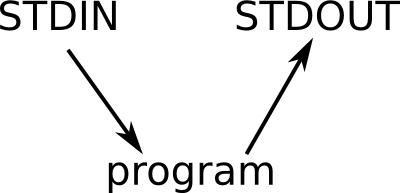
\includegraphics[width=4cm]{asset/g1.png}
\end{figure}
\end{frame}

\begin{frame}[fragile]
\frametitle{Penjelasan Tentang STDIO (lanj.)}
\begin{itemize}
  \item Untuk lebih memahami tentang hal ini, coba buat sebuah berkas bernama input.txt pada \textit{folder} yang sama dengan program jumlah.cpp, dan berisi:
  \begin{lstlisting}
    1
    2
  \end{lstlisting}
  \item Kemudian pada \textit{command line}, saat menjalankan program jumlah.cpp, ketikkan perintah:
  \begin{lstlisting}
    jumlah < input.txt > output.txt
  \end{lstlisting}
  \item Buka output.txt dan perhatikan apa yang tercetak!
\end{itemize}
\end{frame}

\begin{frame}[fragile]
\frametitle{Penjelasan Tentang STDIO (lanj.)}
\begin{itemize}
  \item Isi dari output.txt adalah:
  \begin{lstlisting}
    masukkan nilai a:
    masukkan nilai b:
    hasil dari penjumlahan a dan b: 3
  \end{lstlisting}
  \item Tulisan "masukkan nilai ..." juga ikut tercetak, karena pada kasus ini, \textbf{STDOUT} merupakan berkas output.txt. Segala yang dicetak lewat saluran \textbf{STDOUT} akan dicetak ke output.txt.
  \item Dengan pemahaman yang sama, seluruh masukan yang diberikan adalah lewat \textbf{STDIN}, yang merupakan input.txt. Sehingga masukannya perlu dimasukkan ke input.txt terlebih dahulu.
\end{itemize}
\end{frame}

\begin{frame}
\frametitle{Masukan dan Keluaran pada OSN/IOI}
\begin{itemize}
  \item Setelah kalian memahami tentang \textbf{STDIN} dan \textbf{STDOUT}, mungkin kalian sudah bisa menebak kenapa pada OSN/IOI tidak boleh mencetak informasi masukan seperti "masukkan nilai ...".
  \item Hal ini dikarenakan tulisan itu akan ikut tercetak sebagai keluaran, yang mana mengakibatkan ada keluaran yang tidak sesuai spesifikasi soal. Hasilnya, program akan dinilai \alert{\textit{wrong answer}}, alias menghasilkan jawaban yang tidak sesuai.
\end{itemize}
\end{frame}

\begin{frame}
\frametitle{Selanjutnya...}
\begin{itemize}
  \item Kini kalian sudah mempelajari tentang variabel, ekspresi, dan masukan/keluaran.
  \item Artinya, sudah waktunya untuk menulis program-program sederhana.
\end{itemize}
\end{frame}

\end{document}
